% THIS IS AN EXAMPLE DOCUMENT FOR VLDB 2012
% based on ACM SIGPROC-SP.TEX VERSION 2.7
% Modified by  Gerald Weber <gerald@cs.auckland.ac.nz>
% Removed the requirement to include *bbl file in here. (AhmetSacan, Sep2012)
% Fixed the equation on page 3 to prevent line overflow. (AhmetSacan, Sep2012)

\documentclass{vldb}
\usepackage{graphicx}
\usepackage{balance}  % for  \balance command ON LAST PAGE  (only there!)
\usepackage{cite}
\usepackage{caption}
\usepackage{subcaption}
\usepackage{alltt}
\usepackage[hidelinks]{hyperref}
\usepackage{algpseudocode}
\usepackage{algorithm}
\bibliographystyle{unsrt}
\usepackage{amssymb}
%\usepackage[moderate]{savetrees}
\usepackage{amsmath}
\usepackage{booktabs}
\usepackage[table]{xcolor}
\usepackage{array}
\usepackage{listings}

\begin{document}

% ****************** TITLE ****************************************

\title{Multi-view optimization in key-value stores}

% possible, but not really needed or used for PVLDB:
%\subtitle{[Extended Abstract]
%\titlenote{A full version of this paper is available as\textit{Author's Guide to Preparing ACM SIG Proceedings Using \LaTeX$2_\epsilon$\ and BibTeX} at \texttt{www.acm.org/eaddress.htm}}}

% ****************** AUTHORS **************************************

% You need the command \numberofauthors to handle the 'placement
% and alignment' of the authors beneath the title.
%
% For aesthetic reasons, we recommend 'three authors at a time'
% i.e. three 'name/affiliation blocks' be placed beneath the title.
%
% NOTE: You are NOT restricted in how many 'rows' of
% "name/affiliations" may appear. We just ask that you restrict
% the number of 'columns' to three.
%
% Because of the available 'opening page real-estate'
% we ask you to refrain from putting more than six authors
% (two rows with three columns) beneath the article title.
% More than six makes the first-page appear very cluttered indeed.
%
% Use the \alignauthor commands to handle the names
% and affiliations for an 'aesthetic maximum' of six authors.
% Add names, affiliations, addresses for
% the seventh etc. author(s) as the argument for the
% \additionalauthors command.
% These 'additional authors' will be output/set for you
% without further effort on your part as the last section in
% the body of your article BEFORE References or any Appendices.

\numberofauthors{3} %  in this sample file, there are a *total*
% of EIGHT authors. SIX appear on the 'first-page' (for formatting
% reasons) and the remaining two appear in the \additionalauthors section.

\author{
% You can go ahead and credit any number of authors here,
% e.g. one 'row of three' or two rows (consisting of one row of three
% and a second row of one, two or three).
%
% The command \alignauthor (no curly braces needed) should
% precede each author name, affiliation/snail-mail address and
% e-mail address. Additionally, tag each line of
% affiliation/address with \affaddr, and tag the
% e-mail address with \email.
%
% 1st. author
\alignauthor
Jan Adler
% 2nd. author
\alignauthor
Kaiwen Zhang
% 3rd. author
\alignauthor
H.-A. Jacobsen
% use '\and' if you need 'another row' of author names
% 4th. author
%\alignauthor Lawrence P. Leipuner\\
%       \affaddr{Brookhaven Laboratories}\\
%       \affaddr{Brookhaven National Lab}\\
%       \affaddr{P.O. Box 5000}\\
%       \email{lleipuner@researchlabs.org}
%% 5th. author
%\alignauthor Sean Fogarty\\
%       \affaddr{NASA Ames Research Center}\\
%       \affaddr{Moffett Field}\\
%       \affaddr{California 94035}\\
%       \email{fogartys@amesres.org}
%% 6th. author
%\alignauthor Charles Palmer\\
%       \affaddr{Palmer Research Laboratories}\\
%       \affaddr{8600 Datapoint Drive}\\
%       \affaddr{San Antonio, Texas 78229}\\
%       \email{cpalmer@prl.com}
}
% There's nothing stopping you putting the seventh, eighth, etc.
% author on the opening page (as the 'third row') but we ask,
% for aesthetic reasons that you place these 'additional authors'
% in the \additional authors block, viz.
%\additionalauthors{Additional authors: John Smith (The Th{\o}rv\"{a}ld Group, {\texttt{jsmith@affiliation.org}}), Julius P.~Kumquat
%(The \raggedright{Kumquat} Consortium, {\small \texttt{jpkumquat@consortium.net}}), and Ahmet Sacan (Drexel University, {\small \texttt{ahmetdevel@gmail.com}})}
%\date{30 July 1999}
% Just remember to make sure that the TOTAL number of authors
% is the number that will appear on the first page PLUS the
% number that will appear in the \additionalauthors section.


\maketitle

\begin{abstract}
Lorem ipsum dolor sit amet, consetetur sadipscing elitr, sed diam nonumy 
eirmod tempor invidunt ut labore et dolore magna aliquyam erat, sed diam 
voluptua. At vero eos et accusam et justo duo dolores et ea rebum. Stet 
clita kasd gubergren, no sea takimata sanctus est Lorem ipsum dolor sit 
amet. Lorem ipsum dolor sit amet, consetetur sadipscing elitr, sed diam 
nonumy eirmod tempor invidunt ut labore et dolore magna aliquyam erat, 
sed diam voluptua. At vero eos et accusam et justo duo dolores et ea 
rebum. Stet clita kasd gubergren, no sea takimata sanctus est Lorem 
ipsum dolor sit amet. 


\end{abstract} 


\section{Introduction}
\label{sec:introduction}

%Context
Today's large scale internet services (e.g. Google Maps, Facebook, 
Amazon, etc.) handle millions of client requests, producing 
terabytes of data on a daily basis~\cite{parikh:facebook}. To handle 
this load, major internet companies have developed distributed 
databases called KV-stores such as Google's BigTable\cite{chang:bigtable},
Amazon's Dynamo~\cite{decandia:dynamo}, Yahoo's
PNUTS~\cite{cooper:pnuts}, Apache's HBase~\cite{george:hbase} and
Cassandra~\cite{hewitt:cassandra} (originally Facebook).

KV-stores are highly available to the user and provide advanced 
features like automated load balancing and fault tolerance. KV-stores 
scale horizontally -- by partitioning data and request load across a 
configurable number of nodes. To achieve these properties at a large-scale, 
KV-stores sacrifice an expressive query language and data model, only 
offering a simple API, comprising of \textit{put}, \textit{get} and 
\textit{delete} operations. While this API provides efficient access 
to single row entries, the processing of more complex (SQL-like) queries, e.g. 
selection, aggregation, and join, require costly application-level 
operations. Although, some KV-stores provide additional features to 
support higher-level query processing, those features are often 
rudimentary and impose bottlenecks. 

 Many existing approaches separate transactional and analytical 
processing. A complete snapshot of the data base is copied or loaded to 
an \textit{external} data warehouse and then, processed in a batch-wise 
fashion. Therefore, numerous existing frameworks with varying 
abstraction levels are available, e.g. Map Reduce \cite{dean:mapreduce}, 
Apache Spark \cite{zaharia:spark}, Apache Hive \cite{thusoo:hive}, etc. 
While this approach exploits the benefits of high performance parallel 
processing, it always requires an initial load overhead. Further it is 
not capable of providing up-to-date results -- as frequent changes in 
the base data occur. 

Another way of solving the problem is the use of \textit{internal} 
KV-store mechanisms that directly operate on the KV-store data. Apache 
Pheonix \cite{phoenix:apache} enables rich SQL 
semantics by using the coprocessor functionality (little code snippets, 
deployed on the KV-store nodes) of HBase. While this approach is 
implementation bound to a specific KV-store, we strive for a more general 
solution. 
 

Our approach introduces mechanisms for the materialization and 
incremental maintenance of views to KV-stores. The user 
attains sophisticated query capabilities, simply through definition of 
view expressions. The KV-store keeps results highly available and
enables access of many clients in parallel -- as materialized views 
are simple tables managed in KV-store. Likewise, views can be maintained 
incrementally; only those view records are updated whose 
base records have been changed. The challenge then, is not the scanning
 and computation of base data any more, but the efficient and correct 
maintenance of views. To achieve this at scale, we develop the 
\textit{Distributed View Maintenance System} (VMS) as shown in 
Figure~\ref{fig:research_goal}. The VMS consumes streams of client 
operations (of a base table) and produces the corresponding updates 
(to the view table). 

\begin{figure} 
	\centering 
	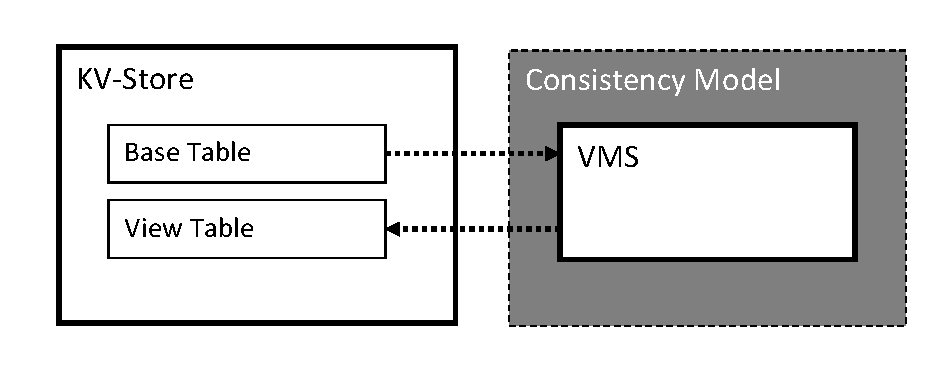
\includegraphics[width=\linewidth]{figures/ResearchGoal} 
	\vspace{-10mm} 
	\caption{System overview} 
	\vspace{-5mm} \label{fig:research_goal} 
\end{figure} 

First, we examine a set of KV-store 
implementations\cite{george:hbase, 
hewitt:cassandra, chang:bigtable, cooper:pnuts} and derive the common 
key characteristics from their architectures and their data models 
(Section~\ref{sec:kv_model}). As is common in the literature on view 
maintenance, we use a consistency model 
(Section~\ref{sec:consistency}) to ensure materialized views remain 
consistent with base data. But unlike the existing 
models\cite{zhuge:view, wang:efficient, zhang:parallel} -- which where 
mainly applied to centralized data warehouse environments -- we design 
our own consistency model to match the needs of a highly distributed 
environment (i.e. KV-stores). Based on the KV-store model and the requirements
of the consistency model, we describe 
the design of the scalable VMS (Section~\ref{sec:view_maintenance_system}). 
We design our VMS to scale in view update load and number of views 
maintained. Our design does not interfere with the read/write processing 
against tables in the KV-store, thus, leaving base table processing 
latencies unaffected. Finally, we conduct a comprehensive 
experimental study (Section~\ref{sec:evaluation}).

% Our approach integrates ``naturally'' with the 
%KV-store: Materialized views are simply tables managed by the store. In 
%spirit with the design philosophy of KV-stores, our approach resorts to 
%incremental and asynchronous view maintenance~\cite{gupta:maintaining, 
%lee:efficient, salem:how}. 

%The VMS is based on the properties and architecture of a typical 
%KV-store -- such as BigTable, HBase, Cassandra, and PNUTS.  



%The correct materialization of views, despite asynchronous and
%concurrent operation processing, is a major concern in the design of VMS.



%That is, only those parts of view tables that 
%are effected as base data changes, are updated. Base updates are 
%propagated asynchronously, not introducing new, costly control 
%dependences into the system. design of our view.  


%We develop a general KV-model in Section~\ref{sec:kv_model}. We adapt
%an existing consistency model in Section~\ref{sec:consistency}. We describe
%the design and behaviour of our View Maintenance System in 
%Section~\ref{sec:view_maintenance_system}.
%our approach.

%Update schema
%Furthermore, we develop a view materialization scheme that avoids 
%expensive table scans and related consistency issues in 
%Section~\ref{sec:view_maintenance}. Our approach supports the 
%maintenance of \texttt{SELECTION}, \texttt{PROJECTION}, \texttt{INDEX}, 
%aggregation (e.g., \texttt{COUNT}, \texttt{SUM}, \texttt{MIN} and 
%\texttt{MAX}), and general \texttt{JOIN} views. To achieve this, we 
%introduce a number of auxiliary view types, such as the \texttt{DELTA}, 
%\texttt{PRE-AGGREGATION} and \texttt{REVERSE-JOIN} view, which are 
%designed to support fast and efficient view maintenance. 



%The correct materialization of views, despite asynchronous and
%concurrent update processing, is a major concern in the design of VMS.
%As is common in the literature on view maintenance, we are using a
%consistency model to ensure materialized views remain consistent with
%base data.  But unlike the existing models\cite{zhuge:view,
%  wang:efficient, zhang:parallel} --- which where mainly applied to
%centralized data warehouse environments --- we design our own consistency
%model in Section~\ref{sec:consistency}, which matches the needs of a 
%highly distributed environment (i.e.  KV-stores). Subsequently, we
%analyse our VMS with regard to the model. While scaling up to hundreds 
%of nodes, fault tolerance becomes a big issue in any distributed system. 
%Thus, we discuss the steps of automatic recovery after crashed components 
%in Section~\ref{sec:fault_tolerance}. Finally, we evaluate our work in 
%Section~\ref{sec:evaluation}, given a 
%full-fledged implementation of the presented concepts based on Apache 
%HBase.  We conduct a comprehensive experimental study that evaluates 
%our approach.



\section{Background}

In \cite{adler_vms}, we showed how materialized views can be
incrementally maintained in a KV-store. Therefore, we developed
an architecture called VMS (cf. Figure~\ref{fig:system_overview}).
Now, we briefly explain the architecture necessary to create and
update view tables in a KV-store.


At the top of Figure~\ref{fig:system_overview}, a general KV-store 
architecture is depicted. It has been derived by looking at various
KV-store implementations (\cite{kv_store1, kv_store2, kv_store3, 
kv_store4, kv_store5}). A KV-store usually comprises a scalable set
of data nodes, each hosting a part of the overall data.  

In Figure~\ref{fig:system_overview} the first node is magnified such that
the write path of the system can be observed. When a client update 
comes in, the client is routed to an appropriate node (e.g. Node~1).
Then, the \textit{client operation} -- in a KV-store it is either a put 
or a delete -- is written to a \textit{transaction log} (TL). The TL
is located on disk and, thus, our extension component (cf. Figure~
\ref{fig:system_overview}) is able to stream the operations from it,
asynchronously. As the figure shows, each node in the KV-store
possesses a TL and an extension component. 


\subsection{KV store}

A KV-store usually  


\begin{figure}[h!] 
	\centering 
	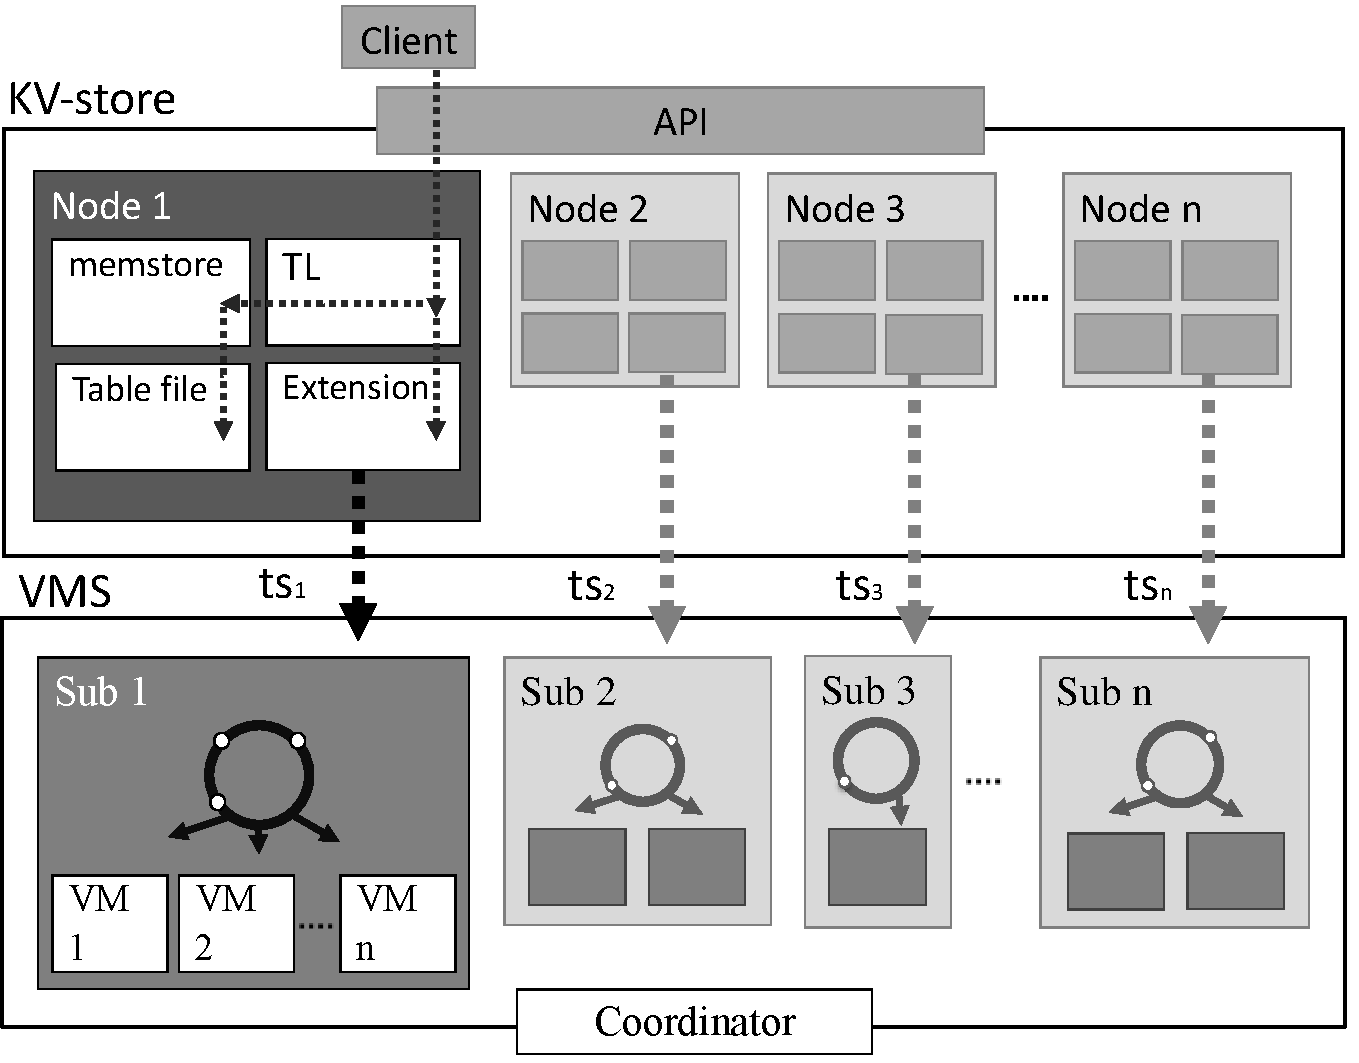
\includegraphics[width=\linewidth]{figures/SystemOverview}  
	\caption{System Overview} 
	\label{fig:system_overview} 
\end{figure} 





The View Maintenance System receives updates from the KV-store in form
of operation streams (see Figure~\ref{fig:system_overview}). Every node
of the KV-store produces a local transaction stream ($ts_1,..,ts_n$);every 
stream of operations is handled by a subsystem of the VMS. The subsystem 
parallizes view update computation: it distributes the updates to a
scalable number of view managers. A view manager actually applies the
update operation to the view table. First, it looks up the view tables 
 defined over the base, then it retrieves the corresponding view record, 
adds the delta to it, and writes back the result to the view.

We express view tables in the VMS with the help of relational algebra 
(e.g., we define a \texttt{SELECTION} as $S=\sigma_{c_1 < x}(A)$ over a 
base table $A$). Defining a view table over a base table is equivalent
to connection the output stream of base table operations with the input
stream of view table input operations. The VMS is also capable of 
defining view tables over view tables (e.g. we define a \texttt{PROJECTION}
view as $P=\pi_{c_1,c_2}(S)$). Thus,
we can concatenate multiple different view types; the VMS will update the
view chain subsequently. It will receive the base table update, apply the
update to the \texttt{SELECTION} view, and apply the result of the first
update to the \texttt{PROJECTION} view.

\section{View expressions}

In this section, we develop techniques for maintaining the following
basic view expressions in our VMS: \texttt{SELECTION}, \texttt{PROJECTION},
\texttt{INDEX}, aggregation (i.e. \texttt{COUNT}, \texttt{SUM},
\texttt{MIN}, \texttt{MAX}, \texttt{AVG}) and join
(i.e. \texttt{INNER}, \texttt{LEFT}, \texttt{RIGHT},
\texttt{FULL}). Internally, VMS provides a number of auxiliary views,
which are the \texttt{DELTA}, \texttt{PRE-AGGREGATION} and
\texttt{REVERSE-JOIN} view, described
shortly. Figure~\ref{fig:view_types} gives an overview of all view
types and their dependencies.




\subsection{Auxiliary views}
\label{subsec:auxiliary_views}

%Reasoning auxiliaries
Auxiliary views are internal to VMS and are not exposed to clients.
They are maintained to enable, facilitate and speed up the correct
maintenance of other view types.  Some views could not be maintained
consistently without the additional information provided by these
auxiliaries, others simply benefit from their pre-computations.  While
auxiliaries introduce storage overhead, they support modularity in 
view maintenance. Logically, auxiliaries represent the basic elements 
of view maintenance, which can be shared within and between view 
definitions. Thus, their use amortizes  as more
complexer views are managed by VMS. Auxiliaries also speed up view 
maintenance significantly. 
The update programs that compute the different view types make up most
of the view manger logic. 

%Auxiliary Table
In what follows, we describe each auxiliary view type, including the 
problem it solves and how it is maintained given base data updates.
In Table~\ref{tab:auxiliary_computation}, the definition, record format
and update operation of the auxiliary views are depicted. In the first
row the base table is shown. The records of the base table correspond
to the general format $r$. A client put (insert or update)
creates an update operation $t_p$, whereas a client delete creates a
$t_d$ operation. As discussed before, the KV-store updates the base
table by itself and provides operations $t_p$ and $t_d$ through the TL. 

\begin{table*}
\rowcolors{2}{gray!10}{gray!30}
\setlength{\belowrulesep}{0pt}
\setlength{\aboverulesep}{0pt}
\setlength\extrarowheight{2pt}
\begin{center}
\begin{tabular}{l l l l l}
\toprule
 & view types & get record & on Insert & on Delete \\
\midrule
1&$A$ & $r=(k,\{\langle c_1,v_1\rangle,..,\langle c_n, v_n\rangle\})$&$t_p=put(r)$&$t_d=delete(k)$  \\
2&$D=\delta(A)$ &  $r'=(k,\{\langle c_1,v_1'\rangle,..,\langle c_n, v_n'\rangle\})$&$put(r)$&$delete(k)$  \\
3&$P=\gamma_{c_{\alpha},\langle K,c_{\beta}\rangle}(D)$ & $p=(v_{\alpha},\{\langle k_1, v_1\rangle,..,\langle k_n, v_n\rangle\})$& $put(v_{\alpha},\{\langle k,v_{\beta}\rangle\})$&$delete(v_{\alpha},\{k\})$  \\
4&$R=\gamma_{c_{\alpha},\langle K,r\rangle,\langle L,s\rangle}$ & $p=(v_{\alpha},\{\langle k_1,r_1\rangle,..,\langle k_n,r_n\rangle \}_A$&$A:put(v_{\alpha}\{\langle k,v_1\rangle\}_A)$&$A:delete(v_{\alpha},\{k\}_A)$  \\
 &$(D_A, D_B)$  & $\{\langle l_1,s_1\rangle,..,\langle l_m, s_m\rangle \}_B)$&$B:put(v_{\alpha},\{\langle k,v_1\rangle\}_B)$&$B:delete(v_{\alpha},\{k\}_B)$ \\
5&$\sigma_{C}(D)$  & $r \lor \emptyset$&$(C)\rightarrow put(r)$&$(C)\rightarrow delete(k,\{c_1,..,c_n\})$  \\
6&$\pi_{c_{\alpha_1},..c_{\alpha_n}}(D)$&  $(k,\{\langle c, v\rangle \mid c \in {c_{\alpha_1},..c_{\alpha_n}}\})$&$put(k,\{\langle c, v\rangle \mid c \in {c_{\alpha_1},..c_{\alpha_n}}\})$&$delete(k,\{c_{\alpha_1},..,c_{\alpha_n}\})$  \\
7&$\gamma_{c_{\alpha},Count(c_{\beta})}(D)$ & $(v_{\alpha},\{\langle c, v_{count}\rangle\})$& $put(v_{\alpha},\{\langle c,v_{count} + 1\rangle\})$&$put(v_{\alpha},\{\langle c,v_{count} - 1\rangle\})$  \\
8&$\gamma_{c_{\alpha},Sum(c_{\beta})}(D)$& $(v_{\alpha},\{\langle c, v_{sum}\rangle\})$& $put(v_{\alpha},\{\langle c,v_{sum} + v_{\beta}\rangle\})$&$put(v_{\alpha},\{\langle c,v_{sum} - v_{\beta}\rangle\})$  \\
9&$\gamma_{c_{\alpha},Min(c_{\beta})}(D)$& $(v_{\alpha},\{\langle c, v_{min}\rangle\})$& $(v_{\beta}<v_{min})\rightarrow put(v_{\alpha},\{\langle c,v_{\beta}\rangle\})$& $(v_{\beta}=v_{min})\rightarrow searchMin()$ \\
10&$\gamma_{c_{\alpha}}(D)$ & $v_{\alpha},\{\langle k_{\alpha},v_{\alpha}\rangle,..\}_A$&$put(\{\langle k,v_1\rangle\}_A)$&$delete(x,\{k\}_A)$  \\
11&$A \bowtie B(R)$& $((k_{\alpha}),\{\langle k_{\alpha},v_{\alpha}\rangle,..\}_A$&$put(\{\langle k,v_1\rangle\}_A)$&$delete(x,\{k\}_A)$  \\
\bottomrule 
\end{tabular}
\caption{Computation table}
\label{tab:kvs_a_events}
\end{center}
\end{table*}
%\begin{table*}
%\rowcolors{2}{gray!10}{gray!30}
%\setlength{\belowrulesep}{0pt}
%\setlength{\aboverulesep}{0pt}
%\setlength\extrarowheight{2pt}
%\begin{center}
%\begin{tabular}{l l l l l}
%\toprule
%View type& Def & record format & on Insert & on Delete \\
%\midrule
%Base &$A$ & $r=(k,\{\langle c_1,v_1\rangle,..,\langle c_n, v_n\rangle\})$&$t_p=put(r)$&$t_d=delete(k)$  \\
%Delta &$D=\delta(A)$ &  $r'=(k,\{\langle c_1,v_1'\rangle,..,\langle c_n, v_n'\rangle\})\lor \emptyset$&$put(r)$&$delete(k)$  \\
%Pre Agg &$P=\gamma_{c_{\alpha},\langle K,c_{\beta}\rangle}(D)$ & $p=(v_{\alpha},\{\langle k_1, v_1\rangle,..,\langle k_n, v_n\rangle\})$& $put(v_{\alpha},\{\langle k,v_{\beta}\rangle\})$&$delete(v_{\alpha},\{k\})$  \\
%Rev Join &$ R=\gamma_{c_{\alpha},\langle K,r\rangle,\langle L,s\rangle}(D_A, D_B)$ & $p=(v_{\alpha},\{\langle k_1,r_1\rangle,..,\langle k_n,r_n\rangle \}_A,..$&$A:put(v_{\alpha}\{\langle k,v_1\rangle\}_A)$&$A:delete(v_{\alpha},\{k\}_A)$  \\
% &  & $\{\langle l_1,s_1\rangle,..,\langle l_m, s_m\rangle \}_B)$&$B:put(v_{\alpha},\{\langle k,v_1\rangle\}_B)$&$B:delete(v_{\alpha},\{k\}_B)$ \\
%\bottomrule 
%\end{tabular}
%\caption{Auxiliary computation}
%\label{tab:auxiliary_computation}
%\end{center}
%\end{table*}
%
%
% 
%\begin{table*}
%\rowcolors{2}{gray!10}{gray!30}
%\setlength{\belowrulesep}{0pt}
%\setlength{\aboverulesep}{0pt}
%\setlength\extrarowheight{2pt}
%\begin{center}
%\begin{tabular}{l l l l l}
%\toprule
%View type & Def & record format & Insert & Delete \\
%\midrule
%Selection &$\sigma_{C}(D)$  & $r \lor \emptyset$&$(C)\rightarrow put(r)$&$(C)\rightarrow delete(k,\{c_1,..,c_n\})$  \\
%Projection &$\pi_{c_{\alpha_1},..c_{\alpha_n}}(D)$&  $(k,\{\langle c, v\rangle \mid c \in {c_{\alpha_1},..c_{\alpha_n}}\})$&$put(k,\{\langle c, v\rangle \mid c \in {c_{\alpha_1},..c_{\alpha_n}}\})$&$delete(k,\{c_{\alpha_1},..,c_{\alpha_n}\})$  \\
%Count &$\gamma_{c_{\alpha},Count(c_{\beta})}(D)$ & $(v_{\alpha},\{\langle c, v_{count}\rangle\})$& $put(v_{\alpha},\{\langle c,v_{count} + 1\rangle\})$&$put(v_{\alpha},\{\langle c,v_{count} - 1\rangle\})$  \\
%Sum &$\gamma_{c_{\alpha},Sum(c_{\beta})}(D)$& $(v_{\alpha},\{\langle c, v_{sum}\rangle\})$& $put(v_{\alpha},\{\langle c,v_{sum} + v_{\beta}\rangle\})$&$put(v_{\alpha},\{\langle c,v_{sum} - v_{\beta}\rangle\})$  \\
%Min &$\gamma_{c_{\alpha},Min(c_{\beta})}(D)$& $(v_{\alpha},\{\langle c, v_{min}\rangle\})$& $(v_{\beta}<v_{min})\rightarrow put(v_{\alpha},\{\langle c,v_{\beta}\rangle\})$& $(v_{\beta}=v_{min})\rightarrow put(v_{\alpha},\{\langle c,v_{x}\rangle\})$ \\
%Index &$\gamma_{c_{\alpha}}(D)$ & $v_{\alpha},\{\langle k_{\alpha},v_{\alpha}\rangle,..\}_A$&$put(\{\langle k,v_1\rangle\}_A)$&$delete(x,\{k\}_A)$  \\
%Join &$A \bowtie B(R)$& $((k_{\alpha}),\{\langle k_{\alpha},v_{\alpha}\rangle,..\}_A$&$put(\{\langle k,v_1\rangle\}_A)$&$delete(x,\{k\}_A)$  \\
%\bottomrule 
%\end{tabular}
%\caption{Standard computation}
%\label{tab:kvs_a_events}
%\end{center}
%\end{table*}



%Reasoning delta view
\noindent  
\textbf{Delta --} The \texttt{DELTA} view is an auxiliary view that 
tracks base table changes between successive update operations. TL 
entries only contain the client operation. They do not characterize the 
base record state before or after the operation. For example, for a 
delete operation, the client only provides the row key, but not the 
associated value to be deleted, as input. Likewise, an update operation 
provides the row key and new values, but not the old values to be 
modified. In fact, a TL entry does not distinguish between an insert and 
update operation. However, for view 
maintenance, this information is vital. This motivated us to introduce 
the \texttt{DELTA} view. It records base table entry changes, tracking 
the states between entry updates, i.e., the ``delta'' between two 
successive operations for a given row. Views that derive, have this 
information available for their maintenance operations. Now, we show 
the computation steps of the \texttt{DELTA} view when updated (see 
Table~\ref{tab:auxiliary_computation}).

%Computation delta view
\noindent
\textit{Computation:} The \texttt{DELTA} view is 
defined over the base table as $D_A=\delta(A)$, meaning all operations 
on the base table are forwarded to the view. The format of the records 
in $D_A$ corresponds to $r'$ -- the state of record $r$ before update 
operation $t_d$ or $t_p$ is applied (e.g. $r'$ holds the values that 
$t_d$ deletes; or $r'$ maybe $\emptyset$ if $t_p$ is an insert 
operation). Once $r'$ is retrieved from the \texttt{DELTA} view, $r$ 
becomes the new $r'$. The VMS updates the view accordingly. If the 
client operation was a delete ($t_d$), the VMS also deletes the record 
in the view. 




%Reasoning pre agg view
\noindent  
\textbf{Pre-Aggregation --} The \texttt{PRE-AGGREGATION} view is an 
auxiliary view that prepares the aggregation by already sorting and 
grouping the base table rows. Consecutive aggregation views only need 
to apply their aggregation function, then. Often, an application 
calculates different aggregations over the same aggregation key.  To materialize these
views, VMS must fetch the same record over and over. For \texttt{MIN}
and \texttt{MAX} views, the deletion of the minimum (maximum) in the
view requires an expensive base table scan to determine the new
minimum (maximum).  This motivated us to introduce the
\texttt{PRE-AGGREGATION} view. This view type sorts the base table
records according to the aggregation key, but stores the grouped rows
in a map.

%Computation pre agg
\noindent
\textit{Computation:}The \texttt{PRE-AGGREGATION} view $P$ is defined over the 
\texttt{DELTA} view $D$ (see Table~\ref{tab:auxiliary_computation}). The 
grouping of the view is based on a column name $c_a$ from the base 
records; the table of the view is sorted according to the grouping key 
$v_{\alpha}$. Every record in the view stores a map of key-value pairs 
(row key $k$ and grouping value $v_{\beta}$) -- representing the 
expanded list of grouping values that belong to a grouping key. The VMS 
can collapse this map in a second step to evaluate the count, sum, 
minimum, maximum or average of the grouped values. A pre-aggregation can 
only be defined over a \texttt{DELTA} view; an update may change the 
grouping key and, thus, requires touching the old and the new record in 
the view. 





%Reasoning reverse join view
\noindent  
\textbf{Reverse Join --}  A 
\texttt{JOIN} view is derived from at least two base tables. For an 
update to one of these tables, the VMS needs to query the other base 
table to determine the matching join rows. Only if the join-attribute is 
the row key of the queried base table, can the matching row be 
determined quickly, unless of course, an index is defined on the 
join-attribute for the table. Otherwise, a scan of the entire table is 
required, which has the following drawbacks: (i) Scans require a 
disproportional amount of time, slowing down view maintenance. (With 
increasing table size, the problem worsens.) (ii) Scans keep the nodes 
occupied, slowing down client requests. (iii) While a scan is in 
progress, underlying base tables may change, thus, destroying view data 
consistency for derived views. To address these issues, we introduce 
the \texttt{REVERSE-JOIN} view. It is an auxiliary view that supports 
the efficient and correct materialization of equi joins in VMS. 
\footnote{We are not discussing theta joins with a full join predicate, 
for it is outside the context of this work.} 

 
%computation reverse join view
\noindent
\textit{Computation (2-tables):}
A \texttt{REVERSE-JOIN} view supports the maintenance of a join between 
two tables: $A \bowtie B_{A.c_{\alpha}=B.c_{\alpha}}$, with join key in 
column $c_{\alpha}$ of tables $A$ and $B$. We define the \texttt{REVERSE
-JOIN} view analogous to the \texttt{PRE-AGGREGATION} view (see Table~
\ref{tab:auxiliary_computation}). This opens up
potential for savings in storage and computation; we can just use the 
same view for both view types (if grouping and join key are the same).

To build the view, we use an aggregation function that collects all 
records of a specific join key; the
join key, defined as $c_a$ -- full-filling the same purpose as the 
grouping key before -- becomes the row key of the view. However, in 
contrast to the \texttt{PRE-AGGREGATION} view, the \texttt{REVERSE-JOIN} 
view consumes tuples from two different input tables, namely $D_A$ and 
$D_B$. When updates are propagated, the
\texttt{REVERSE-JOIN} view can be accessed rapidly from either side of the
relation (the join key is always included in both
tables' updates). If a record is inserted into one of the underlying
base tables, it is stored into the view --- whether it has a
matching row in the join table or not. We are using column families $\{..\}A$ and $\{..\}B$ in the view
to distinguish updates from different base tables. Later, this
facilitates the computation of the matching join rows, for we only
need to build the cross product between the records of the families.  Thus, \texttt{INNER}, 
\texttt{LEFT}, \texttt{RIGHT}, and \texttt{FULL JOIN} can derive from the 
\texttt{REVERSE-JOIN} view without the need for base table scans, as 
we show below.  We discussed the \texttt{REVERSE JOIN} with two join 
tables and a single join key. When increasing the number of join tables
to $n$,  we distinguish two cases:   

(i) Join all tables on the same join key: we just need to extend the
prior definition to $n$ tables. For every new join table $\Phi$ with \texttt{DELTA} view
$D_{\Phi}$, a new column family is added to the view. This column
family collects the updates of the base table.  As long as we are
joining on the same key, we can put all relations to the same
\texttt{REVERSE-JOIN} view.

(ii) base tables are joined on different join keys: for
example, $A \bowtie B \bowtie C$, where table $A$ and $B$ are joined
on column $c_1$, whereas table $B$ and $C$ are joined on a column
$c_3$.  To enable this, we have to combine multiple
\texttt{REVERSE-JOIN} views. We are free to choose, whether we build a
\texttt{REVERSE-JOIN} for $A \bowtie B$ and combine the result with
$C$ or we build a \texttt{REVERSE-JOIN} for $B \bowtie C$ and combine
it with $A$. For every pair of distinct join keys, we need a
\texttt{REVERSE-JOIN} view.  In the worst case, we have $n$ join
tables and $n-1$ distinct join keys, resulting in the same number of
\texttt{REVERSE-JOIN} views.  However, this compositional manner of
deriving join views, leads to a number of possible optimizations. When
computing join $A \bowtie B \bowtie C$ and $B \bowtie C \bowtie D$,
relation $B \bowtie C$ only needs to be computed once, for instance.



\subsection{Standard views}
\label{subsec:common_views}




In this section, we describe how VMS maintains client-exposed views
for a number of interesting standard view types. We also present
alternative maintenance strategies, but defer a full-fledged cost
analysis to future work.

\noindent  
\textbf{Selection and Projection --} A \texttt{SELECTION} view selects
a set of records from a base table based on a \textit{selection
  condition}.  The row key of the base table serves as the row key of
the view table and a single base record uniquely maps to a single view
table record.  A record delete is performed for every operation on the view.  This is
because, the selection condition cannot be evaluated on the operation,
as it may not contain the value.  For $t_d$, the VM does not know the
deleted value and cannot determine, if there is a corresponding view
record. For $t_p$, the VM is not able to distinguish between an insert
vs. an update.  Thus, in both cases, the VM pre-emptively deletes the
record in the view.




A \texttt{PROJECTION} view selects a set of columns from a base
table. Similar to the \texttt{SELECTION} view, the VM uses the row key
of the base table as row key for the view table.  
The computation of the \texttt{PROJECTION} view changes analogously
when derived from a \texttt{DELTA} view. To save storage and
computation resources, we could combine \texttt{DELTA},
\texttt{PROJECTION} and \texttt{SELECTION} into one view. This would
reduce the amount of records (due to selection), the amount of columns
(due to projection), and still provide delta information to subsequent
views. These considerations are important for multi-view optimization
in VMS, which we defer to future work.


\noindent  
\textbf{Count and Sum --} The maintenance of \texttt{COUNT} and
\texttt{SUM} views is very similar, so we treat them together.
Generally speaking, in aggregation views, records identified by an
\textit{aggregation key} aggregate into a single view table record.
The aggregation key becomes the row key of the view. Let a base table
$A$ and $D$ be defined as before. Then, a \texttt{SUM} view is defined
as $S=\gamma_{c_1,Sum(c_2)}(D)$. Note, the view is defined over a
delta table and not a base table. The row key of table $S$ is the
aggregation key of the view (i.e. the value of $c_1$).  Operations
$d_i,\;d_u$ and $d_d$ are processed as follows: The view manager
queries $S$ to retrieve the last state of the aggregated value, e.g.,
$S(v_1',\{\langle c_s,v_s'\rangle\})$. Then, the VM computes the new
state of the aggregated value by adding the ``delta'', i.e.,
$v_s=v_s'+(v_2 - v_2')$. In case the update operation changed the
aggregation key (i.e., $v_1' \neq v_1$), the update involves two
records in the view table. Thus, the VM executes a delete on the old
key $v_1'$ and an insert on the new key $v_1$. A \texttt{COUNT} view
is a special case of a \texttt{SUM} view. Updates for it results by
setting $v_2=1$ and $v_2'=1$ in the following updates for
\texttt{COUNT}:


\textbf{Index --} \texttt{INDEX} views are important to provide fast
access to arbitrary columns of base tables. The view table uses the
chosen column as row key of the view, storing the corresponding table
row keys in the record value. If the client wishes to retrieve a base
table row by the indexed column, it accesses the \texttt{INDEX} view
first, then, it accesses the base table with the row keys retrieved
from the record found in the view. This is a fast type of access, for
the client is always accessing single rows by row key. The
\texttt{INDEX} view is a special case of the \texttt{PRE-AGGREGATION}
view. If the indexed key is the same as the aggregation key, we can
combine both view types. Further, the \texttt{PRE-AGGREGATION} can be
combined with a \texttt{REVERSE-JOIN} view (see description above).
Thus, we receive three different view types at the cost of one.
 
\noindent  
\textbf{Min and Max Views --} \texttt{MIN} and \texttt{MAX} views are
also aggregates. Both can be derived from a \texttt{DELTA} or a
\texttt{PRE-AGGREGATION} view. When derived from a \texttt{DELTA}
view, \texttt{MIN} and \texttt{MAX} are computed similar to a
\texttt{SUM}. However, a special case is the deletion of a minimum
(maximum) in a \texttt{MIN} (\texttt{MAX}). In that case, the new
minimum (maximum) has to be determined. Without the assistance of
auxiliary views, a table scan would have to be
performed~\cite{jacobsen:viewmaintenance}. This motivated us to derive
the \texttt{MIN} (\texttt{MAX}) from a \texttt{PRE-AGGREGATION}, which
prevents the need for a scan.  


\subsection{Joins}
\label{subsec:common_views}


\noindent
\textbf{Join --} The \texttt{JOIN} view presents the results of $n$ 
joined base tables. Since the matching of join partners has been already 
completed in the \texttt{REVERSE JOIN} view, the \texttt{JOIN} view is 
used to display results in a proper way. To get the join result, the VM 
takes the output operations of the \texttt{REVERSE JOIN} view and 
multiplies their column families. Thereby, the \texttt{INNER}, 
\texttt{LEFT}, \texttt{RIGHT}, \texttt{FULL} join can be constructed. 





\section{Maintenance plan}


\subsection{DAG}

We define a maintenance plan as directed acyclic graph (DAG). We denote
the graph as $G=(V,G)$, where every vertex $v \in V$ corresponds to a 
base table or a materialized view and every edge $e \in E$ corresponds to a 
computation, e.g. $\sigma(A)$. The client operations flow from the origin of 
the graph, i.e. the base table, over the edges to the materialized views. The 
edge transforms the input stream into updates for subsequent views. Vertices 
without outgoing edges represent views that deliver the result to the client.

	
\textbf{Example --} 
Consider a client issuing the following query to the View Maintenance System:

\begin{verbatim}
	SELECT Sum(c2) FROM a GROUP BY c_1 WHERE c2 < 10
\end{verbatim} 

In the first naive approach the VMS translates every clause of the
query into a materialized view. The materialized views are concatenated
to build the final result of the query. The client can access the last
view to fetch the results. To 

\begin{figure}[h!] 
	\centering 
	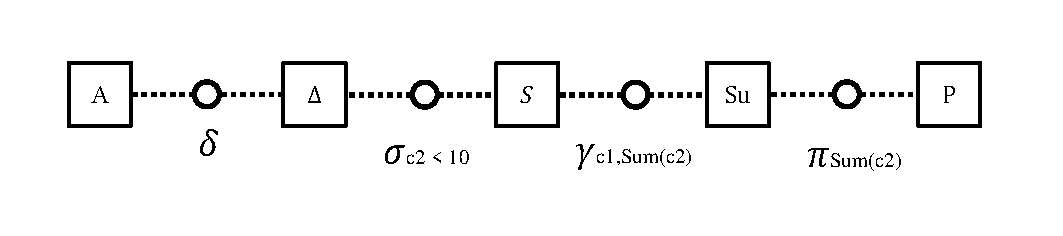
\includegraphics[width=\linewidth]{figures/MaintenanceExample}  
	\caption{Maintenance plan} 
	\label{fig:maintenance_plan} 
\end{figure} 

\subsection{Cost model}



\textbf{Cost model --} 
	Define node cost(storage)
	Define edge cost


\subsection{Optimization}

\textbf{Reorder operation --} 

	Algorithm reordering

\textbf{Merge operation --} 
	
	Algorithm reordering

The \textit{proceedings} are the records of a conference.
ACM, as well as PVLDB, seeks to give these conference by-products a uniform,
high-quality appearance.  To do this, ACM / PVLDB has some rigid
requirements for the format of the proceedings documents: there
is a specified format (balanced  double columns), a specified
set of fonts (Arial or Helvetica and Times Roman) in
certain specified sizes (for instance, 9 point for body copy),
a specified live area (18 $\times$ 23.5 cm [7" $\times$ 9.25"]) centered on
the page, specified size of margins (2.54cm [1"] top and
bottom and 1.9cm [.75"] left and right; specified column width
(8.45cm [3.33"]) and gutter size (.083cm [.33"]).

\subsection{SQL pattern}


The \textit{proceedings} are the records of a conference.
ACM, as well as PVLDB, seeks to give these conference by-products a uniform,
high-quality appearance.  To do this, ACM / PVLDB has some rigid
requirements for the format of the proceedings documents: there
is a specified format (balanced  double columns), a specified
set of fonts (Arial or Helvetica and Times Roman) in
certain specified sizes (for instance, 9 point for body copy),
a specified live area (18 $\times$ 23.5 cm [7" $\times$ 9.25"]) centered on
the page, specified size of margins (2.54cm [1"] top and
bottom and 1.9cm [.75"] left and right; specified column width
(8.45cm [3.33"]) and gutter size (.083cm [.33"]).


\begin{figure}[h!] 
	\centering 
	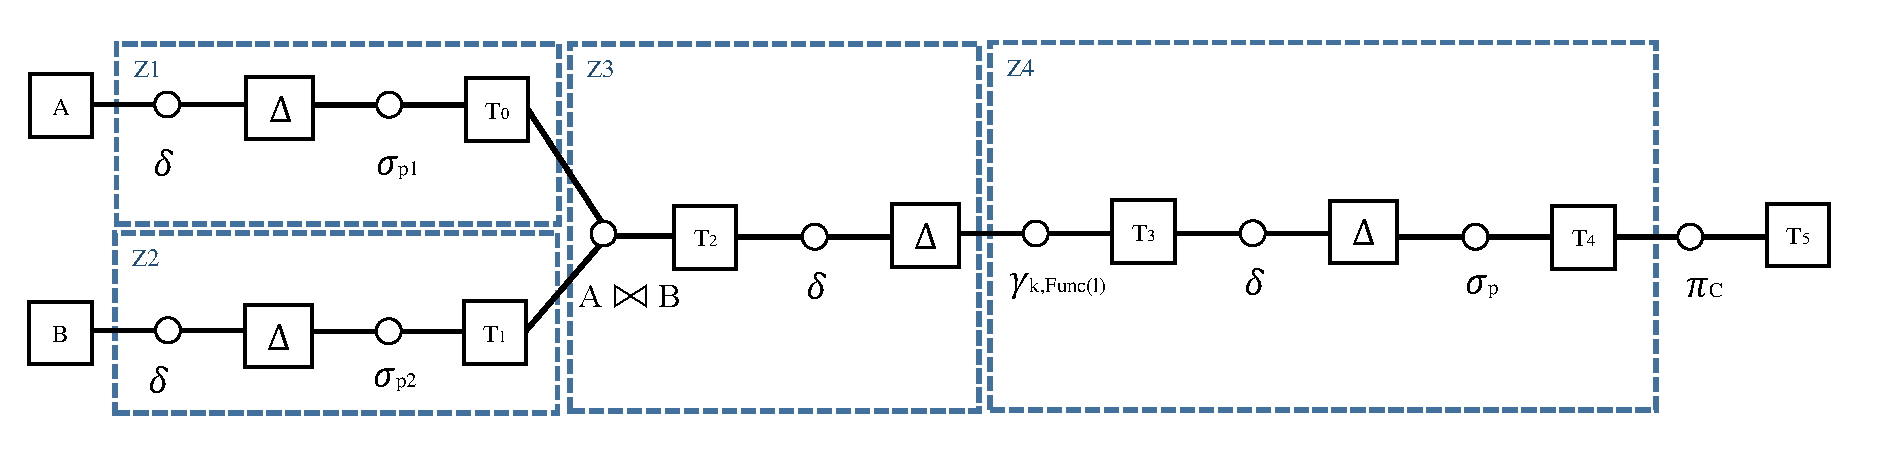
\includegraphics[width=\linewidth]{figures/SQLPattern}  
	\caption{SQL pattern} 
	\label{fig:sql_pattern} 
\end{figure} 

\subsection{Mapping}

	Clauses
	Evaluation order
	Mapping clauses -> view types



\subsection{Optimization}

Reorder
Merge 




The good news is, with only a handful of manual
settings\footnote{Two of these, the {\texttt{\char'134 numberofauthors}}
and {\texttt{\char'134 alignauthor}} commands, you have
already used; another, {\texttt{\char'134 balancecolumns}}, will
be used in your very last run of \LaTeX\ to ensure
balanced column heights on the last page.}, the \LaTeX\ document
class file handles all of this for you.

The remainder of this document is concerned with showing, in
the context of an ``actual'' document, the \LaTeX\ commands
specifically available for denoting the structure of a
proceedings paper, rather than with giving rigorous descriptions
or explanations of such commands.





\section{Multi view optimization}


In the previous sections, we have shown how SQL queries can be 
translated into a query DAG (i.e. maintenance plan). Now, we are ready 
to tackle the multi view problem. Imagine an application or warehousing
system that encounters a large number and variety of different SQL 
queries. Using the naive approach, as described before, would mean
that every query would translate to its own set of materialized views
without sharing any intermediate results. To improve performance and
reduce the storage overhead a lot, we need a query optimizer; the 
optimizer has to find a global maintenance plan which is optimal 
with regard to total throughput and storage usage (or some other cost
parameters). 




\subsection{Cost model}


The cost model has to trade-off the different aspects of incremental
view maintenance. On the one side, there is the throughput of
maintenance operations (which determines the freshness of the data in
the view). A client operation triggers multiple updates along the 
maintenance plan. Depending on the amount and type of view expressions 
a specific number of view updates is generated. On the other side, there 
is the storage cost of hosting the intermediate and resulting view tables. 
The more intermediate tables are hosted, the more storage space is 
occupied. Therefore, we aim at reducing the number of intermediate views 
as much as possible. Whenever, we can possibly execute multiple operations 
on the same table, we combine them.

Both types of cost are expressed in out cost model: the processing or 
maintenance cost and the storage cost. The maintenance cost can be 
described by the number of operations (i.e. get, put and delete) per 
time interval $t$ that the VMS needs to execute to keep the view records 
up-to-date. The rate of operations depends on the view expressions, 
thus, we compute it by iterating over the expression nodes in the 
maintenance plan. First, we define the cost over a single  
vertex $v \in V$ as $c(v)$. The equation is given as follows: 



\begin{equation} 
\begin{aligned} 	   
   c(v)=&\underbrace{(i(v)+u(v)+d(v))*w_g}_\text{get} \\ 
   &+\underbrace{(i(v)+u(v))*w_p}_\text{put} +\underbrace{(d(v)+u(v))*w_d}_\text{delete}
\end{aligned}
\end{equation}

The equation computes the cost of all get, put and delete operations 
that are required to update the subsequent view table. The get part sums 
all get operations and multiplies them with $w_g$, which is a weight 
factor. For all incoming operations, a get-operation has to be performed 
on the view table. This way, the VM retrieves the old view record such 
that it can add the delta on top of it. In some cases, get operations 
are not needed at all (e.g. if a selection view follows a delta view). 
Then, the get-part of the equation can be set to zero. Since KV-stores 
are write optimized data bases -- and, thus, execute writes faster than 
reads -- we also use weight factors $w_p$ and $w_d$ for put and delete 
operations. Update operations can always be substituted by an insert 
plus a delete operation. Thus they are included in the put part, as well 
as the delete part of the equation. 

The functions $i(v)$, $u(v)$ and $d(v)$ deliver the rate of insert, 
update and delete operations that the vertex receives from all its 
direct predecessors. Since the predecessors are table or expression 
nodes, whose input, again, may depend on preceding nodes, we define the 
input rate $i(v)$ recursively. 



\begin{equation} 
\begin{aligned} 	   
	i(v)=& \sum_{v \in pred(v_x)}&i(v)\;\;\; if \; pred(v) \neq \emptyset \\
	i(v)=& &\lambda_i(v)\;\;\; if \: pred(v) = \emptyset
\end{aligned}
\end{equation}


If the set of predecessors is not empty, the sum of input rates over them
is computed. If the set of predecessors is empty, the node must be a base 
table. Then, function $\lambda_i(v)$ represents the rate of operations that 
are applied to the base table. The input rate at the base tables
is either provided to VMS as a meta parameter or has to be determined in
a test run, before actual view maintenance is performed. The equations
to compute update $u(v)$ and delete $d(v)$ rates can be formulated accordingly.

Having the processing cost evaluated we still need to compute the estimated
maximum storage cost. The following general formula works for all view table
nodes:

\begin{equation} 
\begin{aligned} 	   
   c(v)=r(v)*f(v)
\end{aligned}
\end{equation}

%\prod_{v_x \in pred(v_t)} f(v_x)

The input is a table vertex $v \in V$. The function $r(v)$ evaluates
the number of records in the table. Again, the number of records in 
tables can be defined recursively over the maintenance plan as:

\begin{equation} 
\begin{aligned} 	   
	r(v)=& \sum_{v \in pred(v)}&r(v)\;\;\; if \; pred(v) \neq \emptyset \\
	r(v)=& &\mu(v)\;\;\; if \: pred(v) = \emptyset
\end{aligned}
\end{equation}


\begin{figure*} \centering 
	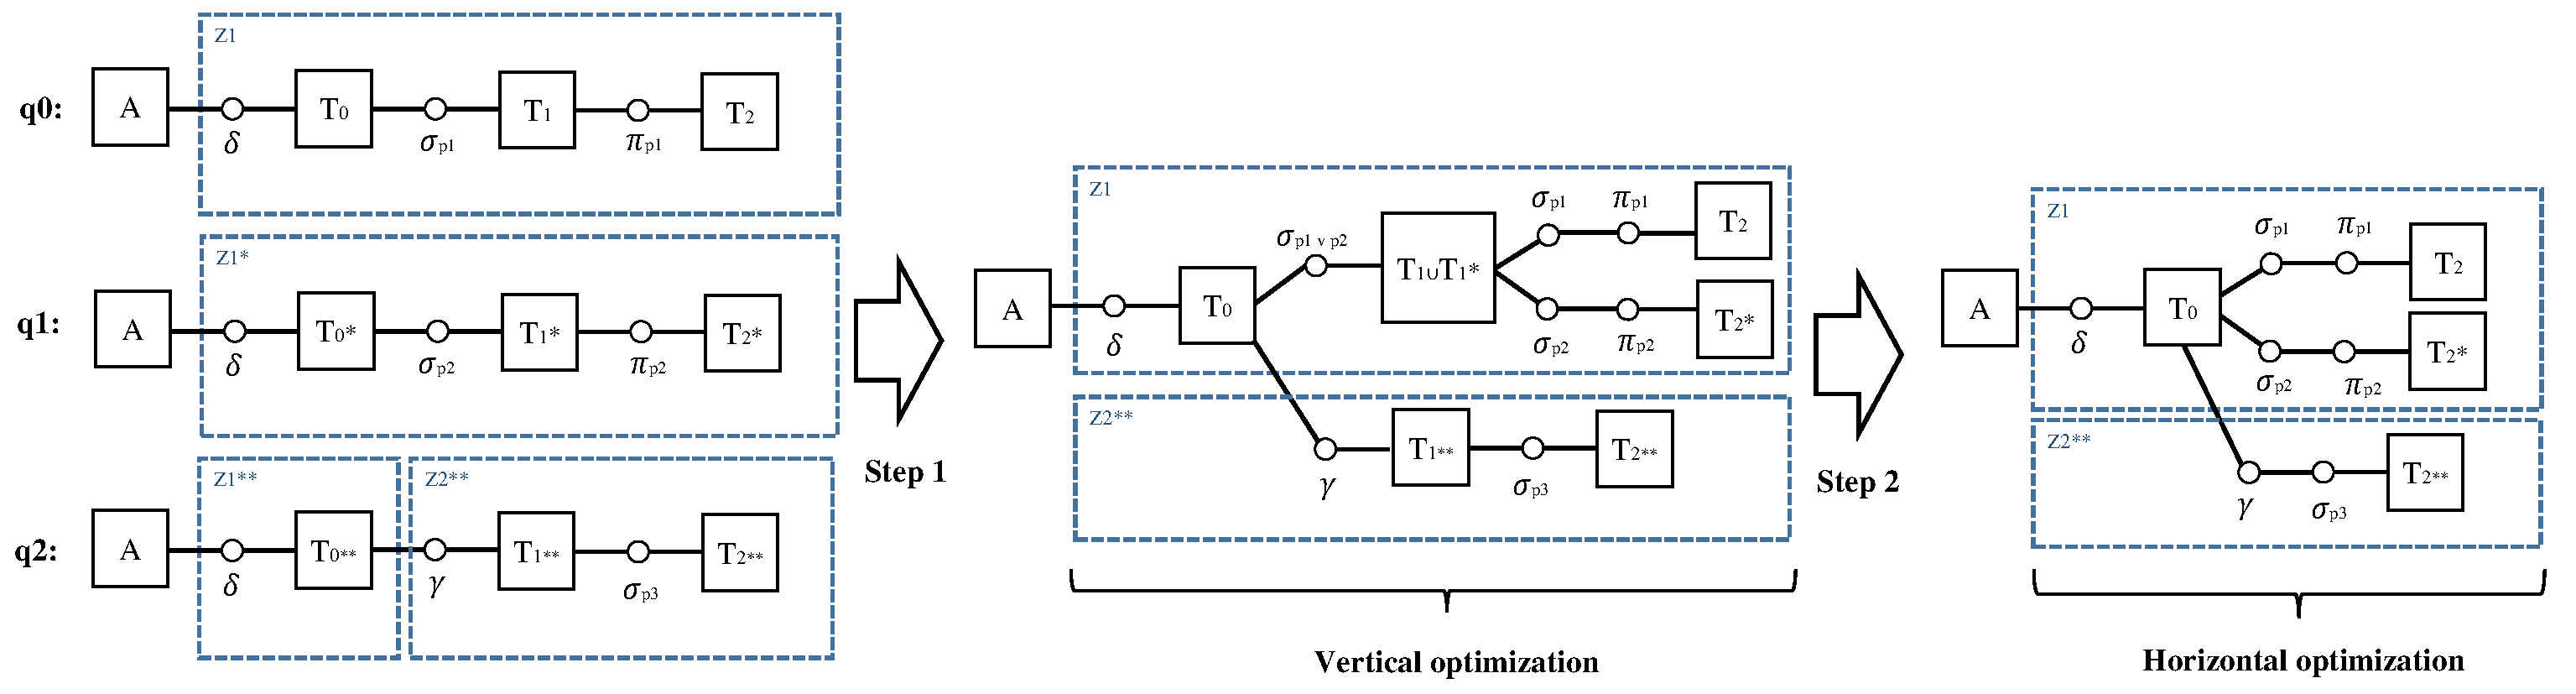
\includegraphics[width=\linewidth]{figures/VerticalOptimization} 
	\caption{Multi-query optimization} \label{fig:vertical_optimization} 
\end{figure*} 

The number of records is defined as the sum of records from the nodes 
predecessors, unless it is a base table. Then,
the function $\mu(v)$ delivers the average number of records. Again, this
number is either given or has to be estimated.
Based on the number of records in the base table, the number of records in 
the view tables can be computed. The number has to be multiplied with a 
factor $f(v)$. The factor expresses that, depending on the view expression,
a the number of view records can be larger or smaller than in the base table.
A selection expression e.g., reduces the amount of records in the view table
depending on the selection predicate. A join can possibly increase the
number of records, e.g. when the cross product of two tables is built. Thus
the function $f(v)$ is denoted as the product of factors from all view 
expressions that are direct predecessors of the node $predX(v)$. The factor, 
represented by function $\psi(v_x)$ has to be given or needs to be evaluated
in a test run.


\begin{equation} 
\begin{aligned} 	   
	f(v)=& \prod_{v_x \in predX(v)}&\psi(v_x)\\
\end{aligned}
\end{equation}


Now, we have defined the cost of table, as well as expression
vertices, we are ready to compute the total cost of the maintenance plan. It is
done as follows:

\begin{equation} 
\begin{aligned} 	   
   c(p)=\sum_{v_x \in V_x(p)} c(v_x)*w_x + \sum_{v_t \in V_T(p)} c(v_t)*w_t
\end{aligned}
\end{equation}

In order to compute the cost of the graph, we need to evaluate the sum 
of the cost of all nodes. Because the cost is based on throughput of client
operations, and nodes are depending on each other (i.e. one node my reduce
the throughput of the next one), the maintenance plan needs to be traversed 
starting at the base tables. Thus, we apply a graph traversing algorithm (e.g. 
Kahn's algorithm) to determine a topology of the graph (i.e. an ordered
according to the placement in the graph). This can be done with linear 
complexity. Then, we follow the topology and compute the throughputs and
storage cost of all nodes iteratively. Finally, we obtain the overall sum
of the maintenance plan $c(p)$.



\subsection{Vertical optimization}

The optimization algorithm operates on a set of query DAGs. In section
before, we merged table nodes within a zone of a single query pattern;
we called it horizontal optimization. Now, we also consider merging table 
nodes of different maintenance plans from different queries; we call it 
vertical optimization.

Figure~\ref{fig:vertical_optimization} depicts the process of vertical 
optimization (and subsequent horizontal optimization). On the left side 
of the figure, three separate maintenance plans of three different 
queries are shown (i.e. $q_0$, $q_1$ and $q_2$). These plans are 
directly derived from the corresponding SQL statements: 



\begin{enumerate}
	\item $q_0$ $\leftarrow$ Select $c_1$ from $A$ where $p_1$ 
	\item $q_1$ $\leftarrow$ Select $c_2$ from $A$ where $p_2$ 
	\item $q_2$ $\leftarrow$ Select Sum($c_2$) from $A$ group by $c_1$ having $p_3$
\end{enumerate}


In Step~1, multiple vertical merges are executed on the plans, which
leads to the graph in the center of the figure. The algorithm starts
at the base tables (i.e. $A$) and merges in a zipper-like fashion 
along the view chain. As a first sub-step all base tables (i.e. all $As$) 
can be merged together. The nodes are identified by name; we take the
first node of $q_1$ as base table node and remove the base table nodes
of $q_1$ and $q_2$. Further, we redirect the outgoing edges of both 
maintenance plans.
As a second sub-step, all delta views (i.e. $T_0$,
$T_0*$ and $T_0**$) are merged together. Since the delta expression 
for all three views is the same, we proceed exactly as before. We
 


\noindent
\textbf{Merging equal expressions}





For the merging of two (or more) table nodes of two (or more) query DAGs,
some preconditions have to be fulfilled: (1) the table node is either
computed from the same expression (e.g. $\sigma_{c_1 = 10}(A)$) or it is
computed from a similar expression of the same operator (e.g $\sigma_{c_1 
< 10}(A)$ and $\sigma_{c_1 > 5}(A)$); thereby, the two expressions need
at least a set of intersection records. Otherwise, it makes no sense to
merge them. (2) the derivation of both tables has to be the same (aside 
from the merged expression). For example, if we merge two aggregation
expressions, then the preceding expressions (e.g. delta, selection) have 
to match exactly.   



Merging equal view tables is always advantageous. Instead of two tables
we just use one, thus, we save storage and processing capacity. 

\noindent
\textbf{Merging similar expressions}


\subsection{Problem definition}

As a first step towards the solution, we formalize the 
problem as follows: 

Given a set of $n$ queries $q_n$ and the corresponding
set of maintenance plans $p_n \in P$: what is the global maintenance
plan $p_g$ that executes all plans $p_n$ and is optimal with 
regard to overall cost.  




\subsection{Optimization algorithm}



Now that we have defined the types of possible merge operations (i.e. 
horizontally and vertically) and also constrained the cost model, we
discuss the optimization algorithm. The first version of our algorithm 
will work in three iterative steps: (1) the algorithm optimizes 
vertically; it finds all equal expressions and table nodes and merges 
them, without cost evaluation. (2) the algorithm optimizes vertically;
it finds all similar expressions and table nodes and merges them based
on cost estimation. (3) the algorithm optimizes horizontally; it uses
the resulting query DAG from the steps before and condenses it further.


\begin{algorithm}
\caption{Multi view optimization}
\label{alg:assignvm}
\begin{algorithmic}[5]
\Procedure{$optimize$}{$P_{Q}$}\Comment{$P_Q$ is a set of plans}
\State $V_G \leftarrow findEqualGroups(P_{Q})$\Comment{Step 1}
\ForAll{$v_g \in V_G$}
\State $P_{Q} \leftarrow verticalMerge(v_g)$	
\EndFor
\State $V_G \leftarrow findSimilarGroups()$\Comment{Step 2}	
\ForAll{$v_g \in V_G$}
\State $benefitial \leftarrow c(verticalMerge(v_g)) < c(v_g) $
\If{$benefitial$}	
\State $P_{Q} \leftarrow verticalMerge(v_g)$
\EndIf	
\EndFor
\State $V_G \leftarrow findZones()$
\ForAll{$v_g \in V_G$}\Comment{Step 3}	
\State $P_{Q} \leftarrow horizontalMerge(v_g)$	
\EndFor
\EndProcedure
\end{algorithmic}
\end{algorithm}


%We define a group as $G=\{{P_Q'}_1..{P_Q'}_n\}$, where $P_Q' \subseteq P_Q$.
%
%\begin{algorithm}
%\caption{Multi view optimization}
%\label{alg:assignvm}
%\begin{algorithmic}[5]
%\Procedure{$optimize$}{$P_{Q}$}\Comment{$P_Q$ is a set of plans}
%
%\State $list_G \leftarrow findCandidateGroups(P_{Q})$\Comment{partitions}
%\ForAll{$g \in list_G$}
%\ForAll{$P_Q' \in g$}
%\If {$mergePossible(P_Q')$}	
%\State $P_Q' \leftarrow verticalMerge(P_Q')$
%\State $P_Q' \leftarrow horizontalMerge(P_Q')$
%\Else
%\State $removeGroup(list_G, g)$	
%\EndIf
%\EndFor
%\If {$c(g) < c(best_g)$}
%\State $best_g \leftarrow g$
%\EndIf
%\EndFor
%
%\Return {$best_g$}
%\ForAll{$v_g \in V_G$}\Comment{Step 3}	
%\State $P_{Q} \leftarrow horizontalMerge(v_g)$	
%\EndFor
%
%
%
%\State $V_G \leftarrow findSimilarGroups()$\Comment{Step 2}	
%\ForAll{$v_g \in V_G$}
%\State $benefitial \leftarrow c(verticalMerge(v_g)) < c(v_g) $
%\If{$benefitial$}	
%\State $P_{Q} \leftarrow verticalMerge(v_g)$
%\EndIf	
%\EndFor
%\State $V_G \leftarrow findZones()$
%
%\EndProcedure
%\end{algorithmic}
%\end{algorithm}


\subsection{Complexity}






\section{Related work}

Research of incremental view maintenance technologies started back in 
the nine-ties. The research was primarily conducted with regard to data 
warehouses \cite{warehouse1, warehouse2, warehouse3, warehouse4}. While 
many principles of incremental maintenance still apply today (e.g. how 
deltas are computed), the underlying architectures have changed 
significantly. The storage capacity has grown, the degree of 
distribution increases continuously. Even though, there was research on 
maintenance of distributed sources \cite{warehouse3}, the warehouse 
itself was a stand-alone system that could be easily queried to retrieve 
information. With the amount of analytical data today multi-view 
optimization becomes a problem. 

Cui and Widom \cite{warehouse1, warehouse2} already examined the usage 
of auxiliary views. Even if the auxiliary views in our context serve a 
different purpose (they define a pre-step of the logical computation), 
they materialized intermediate steps to save processing effort. Already 
here the trade-off of storage vs. processing capacity can be observed. 
However, their research \cite{warehouse1, warehouse2} was more related 
to the problem of lineage tracing and view selection. 

View selection as is also described in \cite{view_selection1, 
view_selection2} is problem, where an algorithm decides, which sub-set 
of a set of view candidates should be materialized. Especially in the 
context of multi-query optimization \cite{multi_query1, multi_query2, 
multi_query3, multi_query4, multi_query5}, it is widely used. However, 
view selection is a different problem than multi-view optimization 
(especially views that are maintained incrementally). In multi-view 
optimization every view has to be materialized. The problem is not the 
choice of the correct materialization set-up, but the reduction of 
processing and storage capacity by resource sharing. 

Even if not the same problem, multi-query optimization (or view 
selection) can provide instruments to also approach the multi-view 
problem. For example, the maintenance plan (e.g. the AND-OR query DAG) 
or a cost model, similar to that of the Volcano optimizer 
\cite{multi_query4, multi_query5} can be used to find an optimal 
solution for the multi-view problem. 

A lot of the modern algorithms for sharing results and optimizing in a 
multi-query environment are based on the map-reduce paradigm 
\cite{map_reduce1, map_reduce2, map_reduce3, map_reduce4}. Map-reduce 
provides a very similar data model to our solution -- records are 
processed in a key-value format. The translation of SQL-statements into 
basic expressions (like selection, aggregation, join) that can share 
elements of computation \cite{map_reduce3} is somewhat comparable to our 
solution. However, the processing style for map-reduce is a 
batch-oriented strategy. Self-contained sets of records are retrieved, 
computed and stored back to disk. When discussing the sharing of 
intermediate results, this problem also reduces to a view selection 
problem. As already stated, our model favours an incremental strategy.
As we are dealing with streams of transactions (as opposed to sets of 
records), optimization algorithms are different. 





\section{Evaluation}

\subsection{Set-up}

\subsection{Work load}

\subsection{Experiments}







% The following two commands are all you need in the
% initial runs of your .tex file to
% produce the bibliography for the citations in your paper.
\bibliographystyle{abbrv}
\bibliography{vldb_sample}  % vldb_sample.bib is the name of the Bibliography in this case
% You must have a proper ".bib" file
%  and remember to run:
% latex bibtex latex latex
% to resolve all references

%\subsection{References}


%APPENDIX is optional.
% ****************** APPENDIX **************************************
% Example of an appendix; typically would start on a new page
%pagebreak

%\begin{appendix}


%\end{appendix}



\end{document}
